\chapter{Testbed}

Per l'implementazione del testbed necessario a eseguire una varietà di test, sono state esaminate numerose schede di sviluppo disponibili sul mercato, caratterizzate da prezzi competitivi e disponibilità immediata. A causa dell'aumento esponenziale dei costi delle varie versioni di Raspberry Pi, soprattutto a seguito della pandemia di Covid-19 e della conseguente scarsità di offerta, si è deciso di escludere a priori queste opzioni.

Inizialmente, si è considerata l'Arduino Yun, una scheda del noto brand Arduino. Tuttavia, si è subito riscontrato che le sue prestazioni erano insufficienti e che gli strumenti forniti non garantivano la flessibilità desiderata. In particolare, la shell risultava poco performante e non era possibile impostare tempi di sleep inferiori a un secondo. Inoltre, è importante notare che l'Arduino Yun è stato deprecato a favore di altre schede, che, sebbene più performanti, non offrivano lo stesso rapporto qualità-prezzo.

Successivamente, si è passati all'analisi di router Mikrotik, ma anche in questo caso le prestazioni e la flessibilità nelle configurazioni non hanno soddisfatto le aspettative.

Alla fine, la soluzione ottimale è stata trovata nelle schede Rock 3 Model A. Queste schede, pur essendo leggermente più economiche rispetto ai Raspberry Pi, offrivano le prestazioni, la flessibilità e il costo contenuto ricercati. Sono state utilizzate quattro unità, tutte configurate in modo identico con Armbian OS come sistema operativo. Ulteriori dettagli verranno forniti in seguito.

Per l'esecuzione delle varie prove, sono stati utilizzati due software: iPerf 2 e Netcat versione OpenBSD.

\section{Rock 3 Model A board}

Il Rock 3 Model A (Figura \ref{fig:rock}) è una scheda di sviluppo avanzata, progettata per applicazioni che richiedono elevate prestazioni di calcolo, rendendola particolarmente adatta per progetti di Internet of Things (IoT), edge computing e server leggeri. 

\begin{figure}[h!]
    \centering
    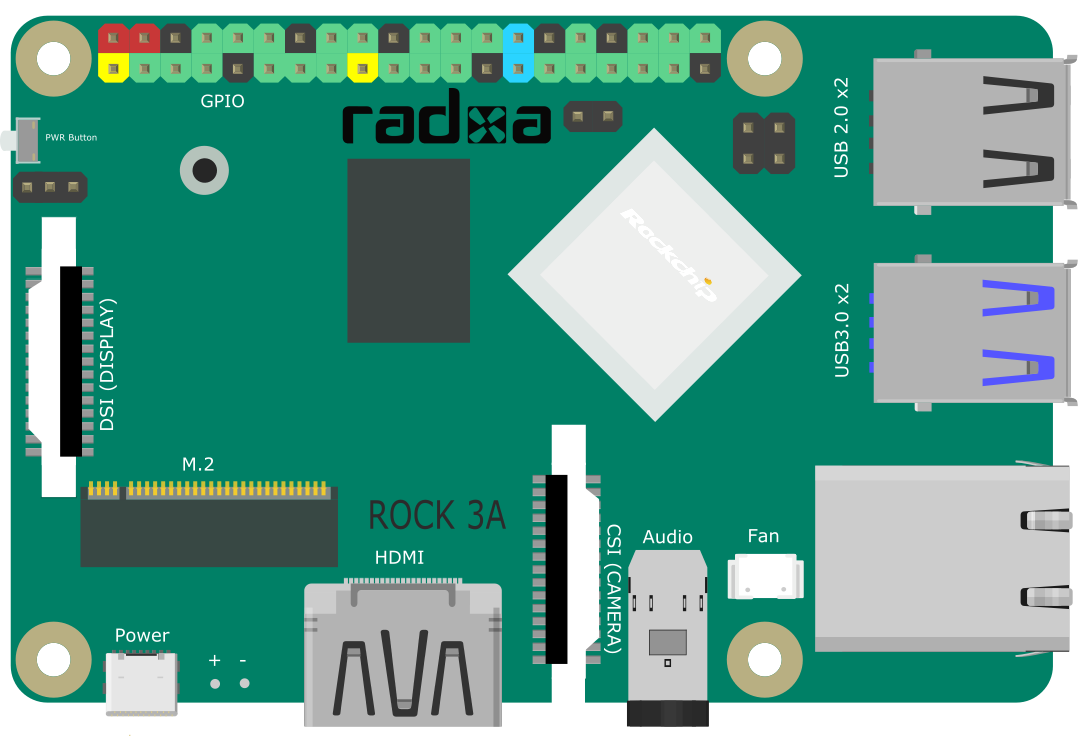
\includegraphics[width=0.7\textwidth]{ROCK_3A.png}
    \caption{Rock 3 Model A}
    \label{fig:rock}
\end{figure}

Al centro di questa scheda si trova il processore Rockchip RK3566, un potente quad-core ARM Cortex-A55 che può raggiungere una frequenza di clock fino a 2.0 GHz. Questa architettura a 64 bit consente di gestire una vasta gamma di applicazioni moderne in modo efficiente. La scheda è dotata di 2 GB di RAM LPDDR4, che garantiscono prestazioni elevate e una gestione efficace delle applicazioni multitasking. Per quanto riguarda l'archiviazione, il Rock 3 Model A offre uno slot per schede microSD, permettendo di espandere facilmente la capacità di memoria, oltre a supportare eMMC fino a 64 GB. Per la connettività, è equipaggiata con una porta Gigabit Ethernet, che assicura una connessione di rete ad alta velocità, e diverse porte USB 3.0 e USB 2.0 per il collegamento di dispositivi esterni. 

Sebbene non sia una caratteristica fondamentale per i nostri scopi, è interessante notare che la scheda include anche una GPU Mali-G52, che consente una buona elaborazione grafica, rendendola adatta per applicazioni multimediali e giochi leggeri. Il Rock 3 Model A offre ampie possibilità di espandibilità, grazie ai pin GPIO (General Purpose Input/Output) che consentono di collegare sensori, attuatori e altri dispositivi. Supporta varie interfacce di comunicazione, come I2C, SPI e UART, facilitando l'integrazione con altri componenti hardware. Per quanto riguarda l'alimentazione, la scheda può essere alimentata tramite un connettore DC o tramite USB-C, offrendo flessibilità nelle opzioni di alimentazione.

La compatibilità con diversi sistemi operativi, tra cui varie distribuzioni Linux come Armbian e Android, rende il Rock 3 Model A estremamente versatile per una varietà di progetti; in particolare, nel nostro caso, si è preferito adottare Armbian OS in quanto risulta essere quello più simile ad un classico sistema \textit{Linux-based} ed inoltre, cosa non di poco conto, fornisce una toolchain comprendente una serie di strumenti e componenti necessari per la compilazione e per il debugging.

\subsection[Atheros Wi-Fi card]{Atheros Wi-Fi card}
Il Rock 3 descritto sopra non monta \textit{out-of-the-box} una scheda di rete che fornisce la connettività Wireless (IEEE 802.11), in virtù di ciò si è reso necessario aggiungerne una esterna collegandola mediante l'interfaccia \textit{PCI Express - M.2 Specification} che la board fornisce per permettere l'espansione delle sue funzionalità hardware.

Tra le varie soluzione in commercio, la scelta è ricaduta sull'adattatore Qualcomm Atheros AR9462. Esso supporta gli standard Wi-Fi 802.11a/b/g/n e permette l'utilizzo della modalità OCB (\textit{Outside the Context of BSS}) utilizzata nel nostro caso al fine di permettere la comunicazione senza fili tra i vari dispositivi senza la necessità di stabilire un \textit{Basic Service Set}.

Un altro aspetto fondamentale che ha reso possibile il nostro lavoro è la possibilità di accedere a una vasta gamma di dati e statistiche sul funzionamento dell'interfaccia di rete, abilitando i flag appropriati durante la compilazione del kernel. Queste informazioni, infatti, non sono generalmente disponibili per la maggior parte delle schede di rete commerciali, rendendo la nostra analisi molto più approfondita e dettagliata. E' possibile accedere a tali statistiche mediante il comando \verb|iw wlp1s0 survey dump| oppure andando ad effettuare un dump dei registri interni della scheda con

\begin{lstlisting}
cat /sys/kernel/debug/ieee80211/phy0/ath9k/regdump
\end{lstlisting}

\noindent Non ci soffermeremo su quest'ultima possibilità in quanto esula dal nostro scopo.

Infine, la natura completamente open-source dei suoi driver ha permesso di apportare ad esso le piccole modifiche necessarie al nostro scopo.

\subsection[Connessione con le board]{Connessione con le board}
Le quattro schede utilizzate nel progetto, come descritto prima, sono dotate di due interfacce di rete distinte, ciascuna con un ruolo specifico nel funzionamento complessivo del sistema. La prima interfaccia è una connessione wireless, utilizzata esclusivamente per l'esecuzione dei test.

La seconda interfaccia è una connessione Ethernet, progettata specificamente per consentire un'interazione diretta con le schede, permettendo così l'invio di comandi per la configurazione, l'avvio e la chiusura dei test, tutti gestiti da un PC.

I quattro dispositivi sono stati collegati a uno switch Ethernet a cinque porte, mentre la porta aggiuntiva è stata riservata per la connessione del PC. Nella figura \ref{fig:etichetta} è mostrata la topologia di rete con i vari indirizzi IP assegnati.

\begin{figure}[h!]
    \centering
    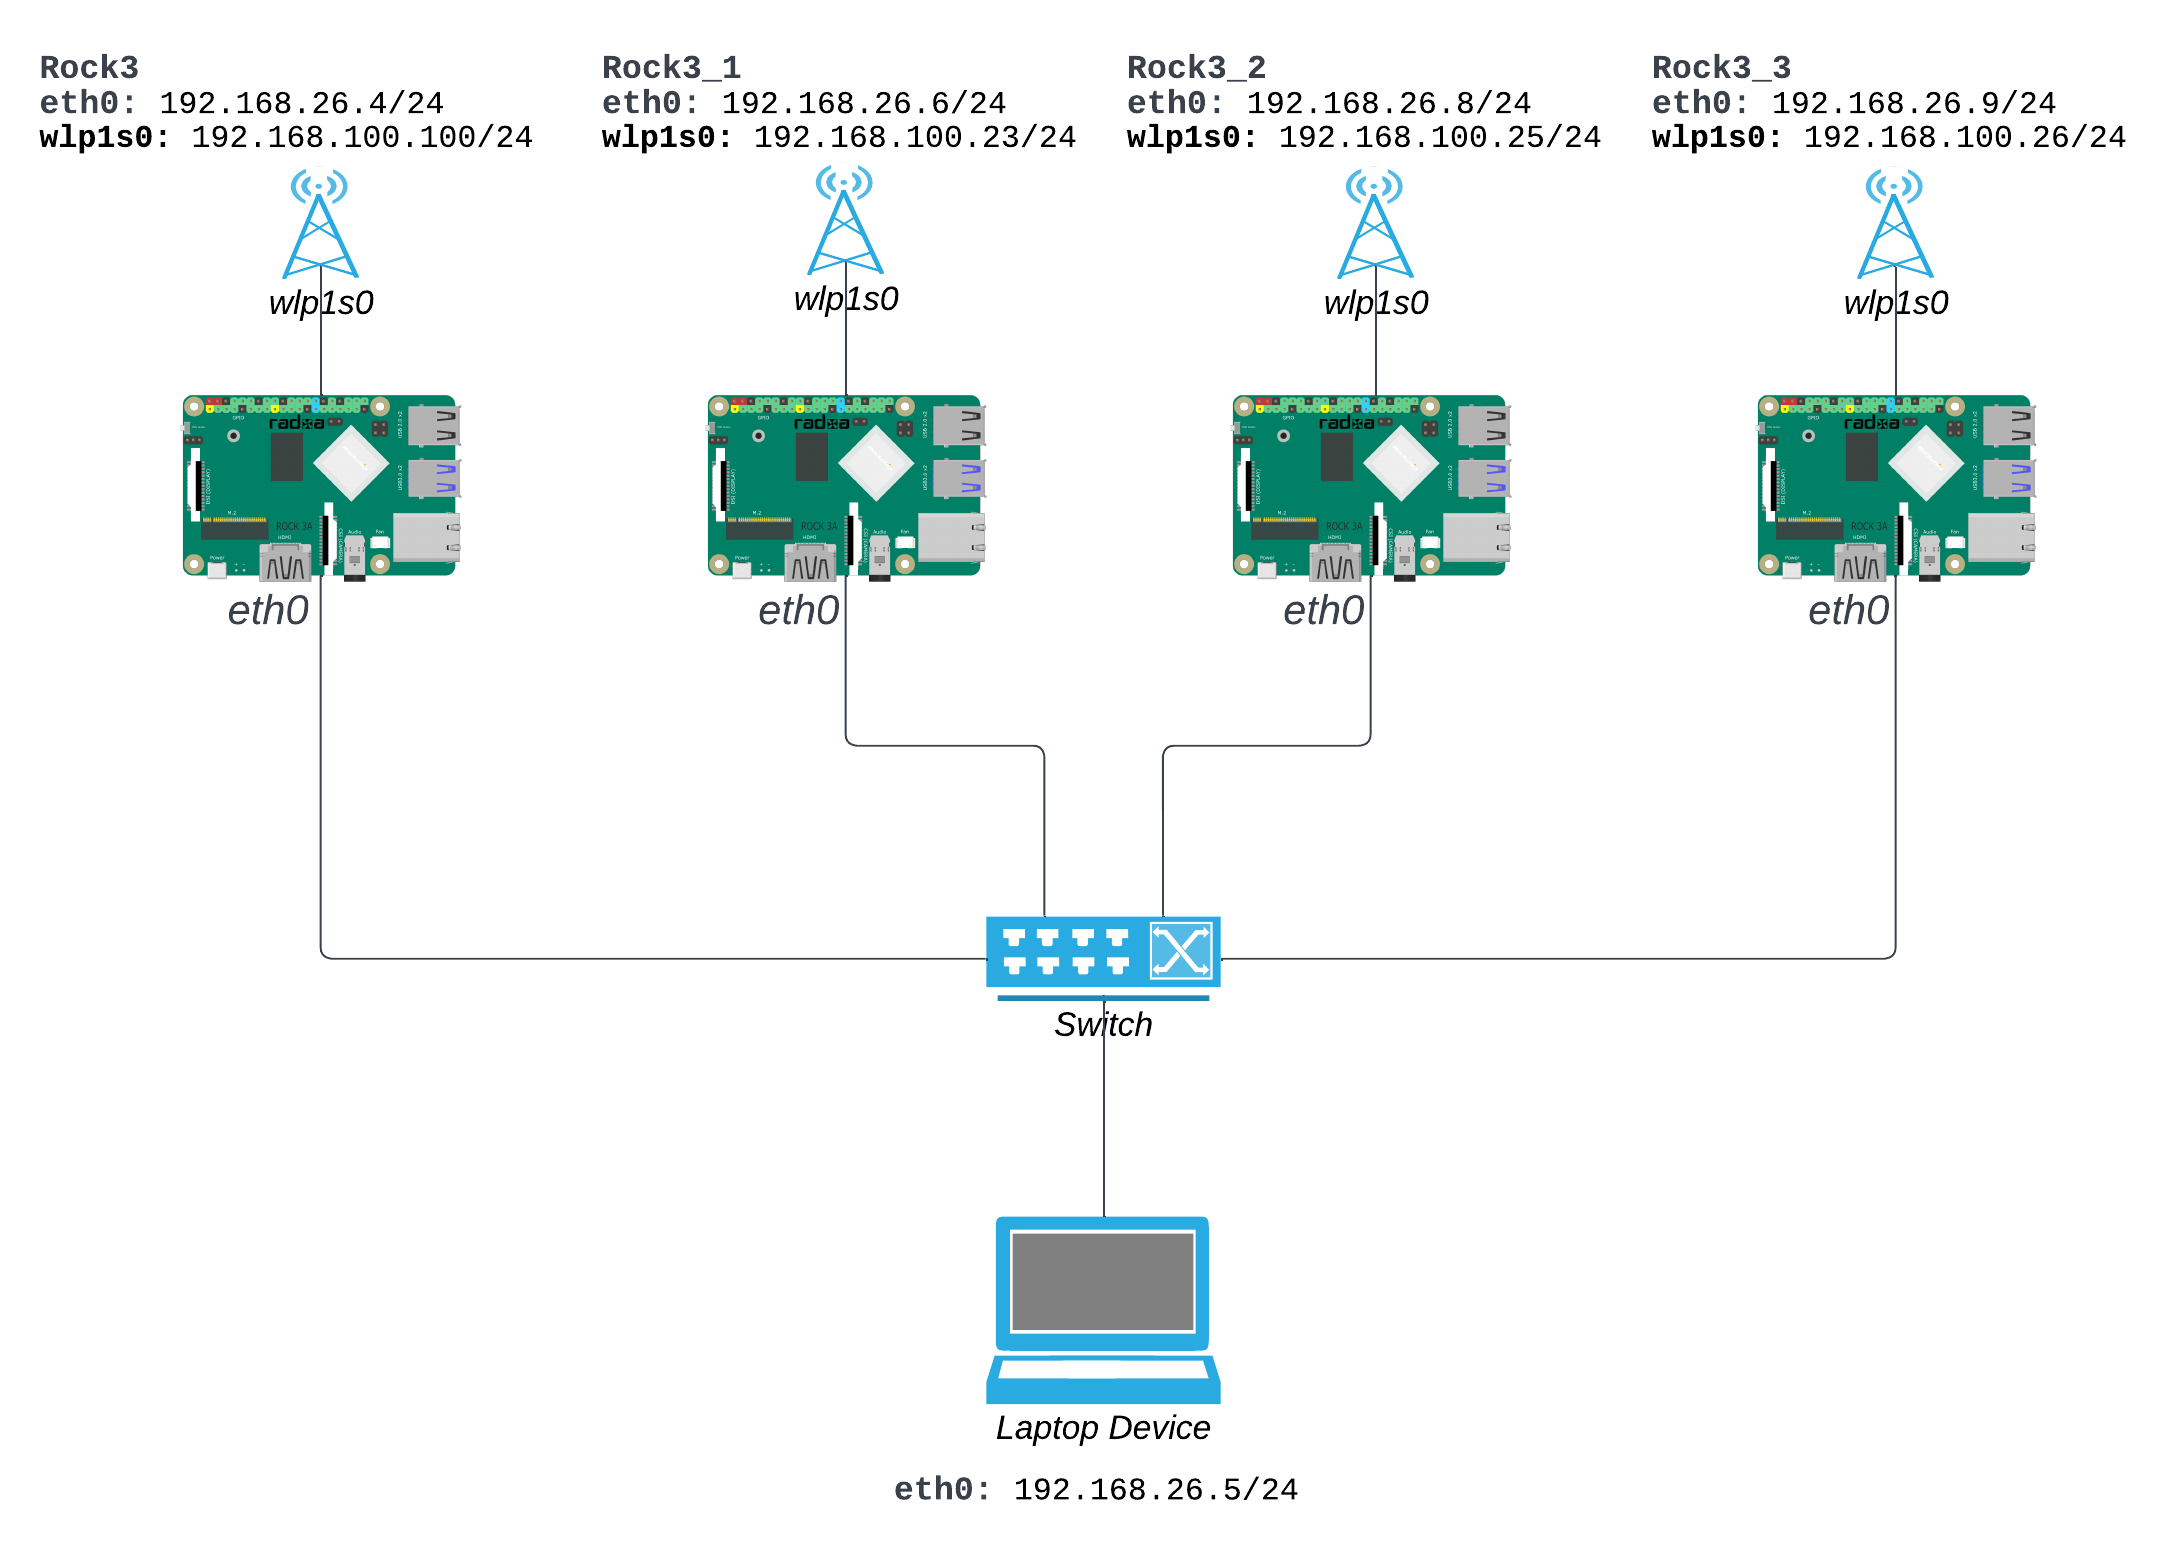
\includegraphics[width=0.7\textwidth]{topology.png}
    \caption{Topologia rete}
    \label{fig:etichetta}
\end{figure}

La connessione avviene mediante il protocollo sicuro SSH, ma non ci si soffermerà su di esso in quanto questo esula dagli obiettivi del presente testo.

\subsection[Impostazione interfaccia Wi-Fi]{Impostazione interfaccia Wi-Fi}
L'interfaccia Wi-Fi di ogni singolo dispositivo Rock, al fine di avere una conessione wireless di tipo OCB funzionante, è stata configurata con i seguenti comandi:

\begin{lstlisting}
    ip link set dev wlp1s0 down
    # imposta la tipologia come ad-hoc
    iw wlp1s0 set type ocb
    # accende l'interfaccia
    ip link set dev wlp1s0 up
    
    iw wlp1s0 ocb join 2462 10MHz
    ip addr add 192.168.100.xxx/24 dev wlp1s0
    ip route add default via 192.168.100.xxx dev wlp1s0
\end{lstlisting}

Non si entrerà nel dettaglio di questi comandi, del resto abbastanza ovvi; ci si limita ad esplicitare che l'interfaccia è stata settata in modalità OCB (\textit{Outside the Context of BSS}), è stato scelto il canale 11, con frequenza fondamentale f\ped{0} pari a 2462 MHz e che, naturalmente, viene assegnato un indirizzo IP con la rispettiva rotta.

Nel nostro progetto, abbiamo deciso di utilizzare una frequenza appartenente alla banda ISM (\textit{Industrial, Scientific and Medical}) anziché quelle specificamente designate dallo standard 802.11p. Questa scelta è stata motivata principalmente dalla necessità di semplificare l'implementazione e garantire la compatibilità hardware.

La banda ISM è ampiamente utilizzata e supportata da numerosi dispositivi commerciali, inclusi quelli a nostra disposizione, il che facilita l'accesso e l'implementazione della tecnologia senza richiedere hardware specializzato. Al contrario, le frequenze stabilite dall'802.11p sono progettate specificamente per le comunicazioni veicolari e richiedono attrezzature più avanzate e costose, che non sempre sono disponibili o compatibili con il nostro sistema.

Inoltre, l'hardware impiegato nel nostro progetto non era completamente compatibile con le frequenze specifiche dell'IEEE 802.11p, il che avrebbe comportato ulteriori complicazioni e ritardi nell'implementazione. L'acquisto di attrezzature adeguate per supportare l'IEEE 802.11p avrebbe comportato un significativo aumento dei costi, rendendo il progetto meno sostenibile dal punto di vista economico.

Optando per la banda ISM, siamo stati in grado di garantire una maggiore interoperabilità e una configurazione più rapida, consentendoci di concentrarci sugli aspetti funzionali del nostro sistema. A livello pratico, questa scelta non comporta sostanziali differenze, se non per il fatto che, lavorando con un canale appartenente alla banda 5.9 GHz avremmo potuto ottenere prestazioni leggermente migliori grazie a una minore congestione della banda. Ciò ci permette di mantenere un sistema efficiente senza dover affrontare le complessità e i costi associati all'implementazione delle specifiche IEEE 802.11p.

\section{Tweaking}
Per rendere possibili alcune configurazioni nei dispositivi Rock e la raccolta dei dati, si è reso necessario mettere mano nalel codice sorgente del Kernel Linux ed applicare alcune patch.

Nella fattispecie, si è dovuto provvedere ad abilitare la \textit{Debug Mode} messa a disposizione dal driver \textit{Ath9k} della scheda di rete wireless ma disabilitata in maniera predefinita, una piccola modifica all'output delle statistiche di rete accessibili dall'utente e l'abilitazione delle code separate per le quattro \textit{Access Categories}.

Tutto ciò è stato reso possibile grazie a patch e a informazioni fornite dalla comunità open source e alla documentazione del produttore.

Viene fornita, inizialmente, una descrizione separata delle varie modifiche apportate, esplicitiando alla fine del trittico il processo di compilazione necessario. Importante notare che le varie patch sono state scritte esclusivamente per la versione del kernel Linux \textit{rockchip64-6.6}, l'ultima disponibile al momento della configurazione del testbed; non si garantisce che possano essere applicate senza ulteriori modifiche ad altre versioni, sia che esse siano sulla architettura ARM che differente.

\subsection[Debug Mode]{Debug Mode}
Per l'abilitazione della suddetta modalità, si è semplicemente messo mano al file \textit{linux-rockchip64-current.config}, file di configurazione utilizzato dalla \textit{toolchain} di compilazione del Kernel del sistema Armbian, abilitando tre differenti flag\cite{linux_wireless}:

\verb|CONFIG_ATH9K_HTC_DEBUGFS=y|

\verb|CONFIG_ATH9K_HWRNG=y|

\verb|CONFIG_ATH9K_DEBUGFS=y|

\subsection[Queues]{Queues}
La patch \textit{00550-ac.patch} fornita modifica un segmento di codice nel file wme.c del driver mac80211, che gestisce la classificazione dei pacchetti in una rete wireless.
Molto semplicemente, si è provveduto ad eliminare la classificazione effettuata dal driver \textit{mac80211} in quanto il suo comportamento andava in conflitto con le Access Categories utilizzate e dirottava tutti i pacchetti sulla coda \textit{Best Effort (BE)}, indipendentemente dalla categoria scelta.
Il problema è dovuto all'introduzione delle cosiddette "code software intermedie" all'interno del driver "mac80211", per i driver supportati\cite{intermediate_queue} come l'\textit{Ath9k}.

\begin{lstlisting}
    --- a/net/mac80211/wme.c        2024-06-17 11:16:29
    +++ b/net/mac80211/wme.c        2024-06-17 11:17:12
    @@ -176,9 +176,9 @@
     
            /* use the data classifier to determine what 802.1d tag the
             * data frame has */
    -       qos_map = rcu_dereference(sdata->qos_map);
    -       skb->priority = cfg80211_classify8021d(skb, qos_map ?
    -                                              &qos_map->qos_map : NULL);
    +       //qos_map = rcu_dereference(sdata->qos_map);
    +       //skb->priority = cfg80211_classify8021d(skb, qos_map ?
    +                                              //&qos_map->qos_map : NULL);
     
      downgrade:
            return ieee80211_downgrade_queue(sdata, sta, skb);
\end{lstlisting}
Questa caratteristica è stata introdotta per spostare l'implementazione delle code più verso il lato software del sottosistema wireless, consentendo all'hardware di mantenere solo code brevi e permettendo anche una maggiore equità tra le stazioni che comunicano.

La possibilità di utilizzare correttamente le categorie di accesso insieme alle code software del \textit{mac80211} risulta essere in fase di implementazione da parte della comunità al momento della stesura di questo elaborato.

\subsection[Statistiche occupazione canale]{Statistiche occupazione canale}
La patch fornita, di nome \textit{00551-ac.patch}, modifica un segmento del codice nel file link.c del driver \textit{ath9k}, che è parte della gestione delle statistiche di monitoraggio della rete wireless. Esso in maniera predefinita restituiva, mediante il comando \verb|iw wlp1s0 survey| \verb|dump|, varie statistiche tra cui i tempi in cui, rispettivamente, il canale risulta essere occupato, viene usato per trasmettere e ricevere da parte dell'interfaccia. 

Questi valori venivano mostrati in output in maniera incrementale, ovvero ogni valore campionato era sommato al valore precedente; tale modus operandi complicava la raccolta dei dati nel nostro caso e si è provveduto a modificare il codice in modo che i valori vengano mostrati, singolarmente, volta per volta.
\begin{lstlisting}
    --- a/drivers/net/wireless/ath/ath9k/link.c	2024-06-21 11:46:11
    +++ b/drivers/net/wireless/ath/ath9k/link.c	2024-06-21 11:47:38
    @@ -524,10 +524,10 @@
                 SURVEY_INFO_TIME_BUSY |
                 SURVEY_INFO_TIME_RX |
                 SURVEY_INFO_TIME_TX;
    -		survey->time += cc->cycles / div;
    -		survey->time_busy += cc->rx_busy / div;
    -		survey->time_rx += cc->rx_frame / div;
    -		survey->time_tx += cc->tx_frame / div;
    +		survey->time = cc->cycles / div;
    +		survey->time_busy = cc->rx_busy / div;
    +		survey->time_rx = cc->rx_frame / div;
    +		survey->time_tx = cc->tx_frame / div;
         }
     
         if (cc->cycles < div)
\end{lstlisting}
Giusto per completezza, viene mostrato l'output dell'esecuzione del comando 

\verb|iw| \verb|wlp1s0 survey dump|:
\begin{lstlisting}
root@rock-3a:~# iw wlp1s0 survey dump
    Survey data from wlp1s0
	frequency:			2462 MHz [in use]
	noise:				-93 dBm
	channel active time:		136546 ms
	channel busy time:		1642 ms
	channel receive time:		1496 ms
	channel transmit time:		0 ms
\end{lstlisting}
Per semplicità viene mostrato qui solo l'output relativo al canale 11, omettendo le informazioni relative agli altri canali.

Per calcolare il carico del canale, ovvero la percentuale di tempo in cui il canale wireless è occupato, sono stati raccolti due valori fondamentali: il \textit{channel active time} e il \textit{channel busy time}. Il primo rappresenta il tempo in cui l'interfaccia è attiva per trasmettere, ricevere o ascoltare il canale, mentre il secondo indica il tempo in cui l'interfaccia è attiva ma in attesa a causa dell'occupazione del canale\cite{han2016adaptive}.
\subsection[Kernel building]{Kernel building}
Per la compilazione dell'intero sistema Armbian o, nello specifico, del Kernel, ci si è basati sulla toolchain messaci a disposizione dalla comunità open source. 

La toolchain di Armbian è una componente essenziale per sviluppare e ottimizzare software per dispositivi ARM, specialmente quando si lavora con macchine host x86. Il cuore di questa toolchain è il compilatore GCC, configurato specificamente per il target ARM. Questo compilatore traduce il codice sorgente in codice eseguibile ottimizzato per le architetture ARM, permettendo di sfruttare appieno le capacità hardware dei dispositivi.

Un suo aspetto cruciale è la cross-compilazione. Lavorare con dispositivi ARM spesso significa confrontarsi con limitazioni di risorse hardware che rendono impraticabile la compilazione diretta. La cross-compilazione risolve questo problema permettendo di compilare il software su una macchina più potente (solitamente un PC x86) e poi eseguirlo sul dispositivo ARM. Questo processo non solo accelera notevolmente la compilazione, ma evita anche il rischio di esaurire le risorse durante la build.

Il sistema di build automatizzato di Armbian gioca un ruolo centrale nella gestione di questo processo. Gli script e gli strumenti inclusi orchestrano la compilazione del kernel, del bootloader e dei vari pacchetti software, assicurando che tutto sia perfettamente integrato e ottimizzato. Questo sistema è pensato per gestire le complessità della cross-compilazione, semplificando il processo per gli sviluppatori.

Non ci si dilungherà nelle modalità di download e installazione di tutto il pacchetto, in quanto è tranquillamente reperibile in rete e richiede, per la sua configurazione iniziale, componenti esterne quali Docker. Una volta installato e funzionante, fatte le modifiche ad-hoc al file di configurazione (il citato precedentemente file \textit{linux-rockchip64-current.config}) ed inserite le patch già menzionate nella cartella

\verb|~/build/patch/kernel/archive/rockchip64-6.6 |

\noindent e si procede alla compilazione mediante il comando 

\verb|./compile.sh kernel ARTIFACT_IGNORE_CACHE='yes' \| 

\verb|BOARD=rock-3a BRANCH=current|

\noindent Il processo restituirà il nuovo kernel pacchettizzato all'interno di file \textit{.deb}, che andranno installati sui dispositivi come di consueto.

\section{iPerf con Access Categories abilitate}
iPerf è un software di benchmarking di rete utilizzato per misurare le prestazioni della larghezza di banda e della latenza nelle connessioni TCP e UDP. Permette di misurare la larghezza di banda disponibile tra due punti di rete, offrendo la possibilità di testare sia il protocollo TCP, orientato alla connessione, sia il protocollo UDP, non orientato alla connessione. Il software funziona in modalità client-server, dove un'istanza di iPerf agisce da server e l'altra da client, permettendo di eseguire test in entrambe le direzioni.

Le modalità con cui tale software è stato utilizzato verranno discusse più avanti nell'apposito capitolo; qui ci si soffermerà, più che altro, sulle modifiche effettuate al codice sorgente.

La patch, che per chiarezza di lettura non è stata inserita in questo paragrafo ma potrà essere trovata in appendice (\autoref{iperf_ac}), abilita il supporto alle 4 code EDCA del livello MAC. L'opzione -A, specifica per iPerf in modalità client, può ora essere usata per specificare una classe di traffico a cui inviare il flusso in uscita (-A BK o -A BE o -A VI o -A VO). Se non si specifica alcuna classe di traffico, le opzioni rimangono quelle di un pacchetto iPerf 2 standard (cioè si utilizza effettivamente AC\_BE).

Da notare che la patch è stata sviluppata per la versione 2 del software (nello specifico la v2.2.0); esiste anche la versione 3 che, tuttavia, non è stata presa in considerazione in quanto i cambiamenti architetturali effettuati al programma non consentivano, facilmente, l'impletazione delle modifiche necessarie.

\section{Netcat OpenBSD}
Netcat, spesso abbreviato in nc, è un potente strumento di rete utilizzato per leggere e scrivere dati attraverso connessioni di rete TCP o UDP. È spesso descritto come "il coltellino svizzero" degli strumenti di rete, grazie alla sua versatilità.

Netcat può essere utilizzato per una varietà di scopi, tra cui il debugging delle connessioni di rete, il trasferimento di file, la creazione di tunnel e la comunicazione tra sistemi. Può funzionare sia in modalità client, per connettersi a un server, sia in modalità server, per ascoltare le connessioni in arrivo su una porta specifica.

Esistono differenti porting e implementazioni; le più importanti sono GNU e OpenBSD; esse sono simili se non per alcune differenze nelle funzionalità offerte e in alcuni parametri di esecuzione disponibili (la versione BSD, per esempio, supporta IPv6, proxy e gli Unix socket che la tradizionale non ha). 

Nel nostro caso, la necessità di dover eseguire il comando netcat col paramentro \verb|-q 0|, ovvero disabilitare l'attesa dopo l'EOF su stdin, ha portato ad utilizzare l'OpenBSD anzichè la tradizionale.